\documentclass[12pt,a4paper,titlepage]{article}
\usepackage[utf8]{inputenc}
\usepackage{amsmath}
\usepackage{algorithm}
\usepackage[noend]{algpseudocode}
\usepackage{amsfonts}
\usepackage{amssymb}
\usepackage{graphicx}
\usepackage{color}
\usepackage{float}
\usepackage[margin=1in]{geometry}
\author{800107 - Daniel Ng See Cheong\\
		839521 - Uzair Moolla}
\title{
	AAA Project\\
	\large Solving Sudoku using the backtracking algorithm
}

\graphicspath{ {images/} }

\newcommand{\todo}[1]{\textcolor{red}{\textbf{\##1\#}}}

\begin{document}
\maketitle

\section{Introduction}
Sudoku is a numerical based logic puzzle game. The idea is to fill in an $n\times n$ grid with numbers in a specific manner. The most commonly known grid usually consists of square blocks with 3 rows and 3 columns. These individual blocks are then arranged in a similar manner again, with 3 blocks along rows and 3 along columns, producing a $9 \times 9$ matrix. An example of this described matrix can be seen in Figure  \ref{fig:Blank_Sudoku_Board}. We need to fill each of the blocks with one of these numbers ${1,2,3,4,5,6,7,8,9}$. The rules for filling these blocks are as follows:
\begin{itemize}
\item[•] Within each $3 \times 3 $ block we can only have single occurrence of each number.
\item[•] Along each $9$ block row we can only have a single occurrence of each number.
\item[•] Along each $9$ block column we can only have a single occurrence of each number.
\end{itemize}

\noindent
An example of a Sudoku Puzzle completed using the rules stated above can be seen in Figure \ref{fig:Complete_Sudoku_Board}.

\begin{figure}[H]
\centering
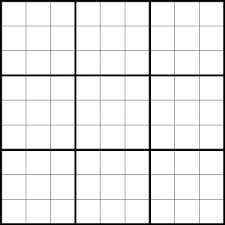
\includegraphics[scale=0.5]{Blank_Sudoku_Board}
\caption{Sample of a $9\times9$ Blank Sudoku Board}
\label{fig:Blank_Sudoku_Board}
\end{figure}
%-------------------------------------------------------%
\begin{figure}[H]
\centering
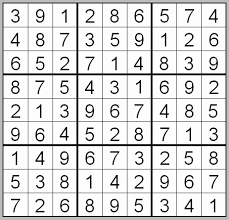
\includegraphics[scale=0.5]{Complete_Sudoku_Board}
\caption{Sample of a $9\times9$ Completed Sudoku Board}
\label{fig:Complete_Sudoku_Board}
\end{figure}
%------------------------------------------------------%

\noindent
Solving sudoku puzzles are a fun exercise for many. However we would like to find a suitable algorithm which can be used to solve sudoku puzzles correctly as well as efficiently. There are various possible methods which can be used to solve sudoku puzzles. We will be focussing on the \emph{Backtracking Algorithm} in our experiments.
\\
\todo{Fill in facts}

\newpage
\section{Aims}

We are going to use the backtracking algorithm to solve sudoku puzzles of size $n\times n$. We will attempt to solve these sudoku puzzles accurately and in as little time as possible. Once we have the algorithm working correctly we will perform both empirical as well as theoretical analysis on it. We aim to find the best, average and worst case complexities of the algorithm being used. These results will be obtained through both methods of analyses (empirical as well as theoretical) and correlations between the results will be obtained.
\\
We will create a database of unsolved puzzles and another with their corresponding solutions. These lists will be used for all analysis done as well as ensuring that the solutions found to each of the puzzles are correct. 
\\
\todo{add some stuff}

\section{Summary of Theory}

\subsection{Backtracking Algorithm}

In general backtracking algorithms are mainly used to solve NP-complete computational problems. Simply put, the backtracking algorithm starts with the selection of one possible move out of all available moves and will try solving the problem with the selected move. If the selected move allows us to find a correct final solution to the problem, the solution is given as an output (it is printed out). However, if the selected move does not lead to a correct final solution to the problem, we backtrack. The backtracking is done to the point where the move was selected and choose an alternative one at this point. This process is repeated until the correct solution to the problem is found. If none of the available moves work in finding the correct solution to the problem it is sufficient to say there is no solution to the problem.
\\
Recursion is the most appropriate method to implement this type of algorithm.
\\
\todo{add more stuff}

\section{Pseudo code}

\begin{algorithm}[H]
\caption{Check if  a Move is Valid}
\begin{algorithmic}

\Function{validMove}{number , row, column}
\\
Where:
\\
\textit{number} is the number to be inserted
\\
\textit{row} is the row of current position
\\
\textit{col} is the column of the current position
\\
\textit{n} is the length of the square matrix representing the sudoku puzzle grid 
\\
\textit{board} is the $n \times n$ square matrix representing the sudoku puzzle grid 
\\

	\For{i from 1 to n}
		\If{number is equal to board[row][i]}	
			\State return false
		\EndIf
	\EndFor 	

	\For{i from 1 to n}
		\If{number is equal to board[i][col]}	
			\State return false
		\EndIf
	\EndFor	
	
	
	\\
	\\
	initialise rowmin to $ \dfrac{row}{blocksize} \times blocksize $
	\\
	\\	
	initialise colmin to $ \dfrac{column}{blocksize} \times blocksize $
	\\
	\\		
	initialise rowmax to (rowmin + blocksize)
	\\		
	initialise colmax to (colmin + blocksize)	
	\\
	
	\For{i from rowmin to rowmax }
		\For{j from colmin to colmax}  	 
			\If{number = board[i][j]}
	   			\State return false
	 		\EndIf       
  		\EndFor
  	\EndFor
	\State return true
\EndFunction
\end{algorithmic}
\end{algorithm}

%---------------------------------------------------------------------

\begin{algorithm}[H]
\caption{Check if a Position is Open}
\begin{algorithmic}
\Function{openPosition}{}
\\
\textit{n} is the length of the square matrix representing the sudoku puzzle grid
\\
\textit{board} is the $n \times n$ square matrix representing the sudoku puzzle grid 
\\ 
\State initialise temp to be an array of length 2
  
	\For{i from 1 to n}
		\For{j from 1 to n}  	 
			\If{board[i][j] is empty}
				\State temp[0] = i
				\State temp[1] = j
				\State return temp 
			\EndIf       
		\EndFor
	\EndFor
	\State  return NULL
\EndFunction

\end{algorithmic}
\end{algorithm}

%----------------------------------------------------------------

\begin{algorithm}[H]
\caption{Backtracking}
\begin{algorithmic}
\Function{solve}{}
\\
\textit{n} is the length of the square matrix representing the sudoku puzzle grid 
\\
\textit{board} is the $n \times n$ square matrix representing the sudoku puzzle grid
\\
\textit{openPosition(),validMove(i,row,col)} are the functions described above in Algorithm 1 and Algorithm 2 respectively.
\\ 
	\State initialise row and col; 
	\State initialise temp to openPosition();	

	\If{temp is not NULL} 
		\State row = temp[0];
		\State col = temp[1];
  	\Else
		\State return true
	\EndIf  
	
	\For{i from 1 to n}
		\If{validMove(i,row,col) is true}
			\State board[row][col]=i;
       		\If{solve() is true}
       			\State return true;
       		\EndIf       
			\State set board[row][col] to be empty;
		\EndIf
	\EndFor
	\State  return false;
\EndFunction

\end{algorithmic}
\end{algorithm}

\section{Theoretical Analysis }

Theoretical analysis will be done for each of the algorithm pseudo codes listed above. However the first two algorithms are used in the Backtracking Algorithm (ie Solve calls validMove as well as openPosition) and thus the analysis of the Backtracking Algorithm will be done taking into account the analysis of Algorithms 1 and 2. We are able to do this as the aim of this experiment is to find the complexity of the Backtracking Algorithm being used to solve a sudoku puzzle.

\subsection{Algorithm 1: validMove}
 
We will use comparisons as the basic operation in this algorithm. There are two main segments in this algorithm, the first simply checks if  the number to be inserted in the puzzle already exists in the row or column of the block we want to insert it into. 

\todo{Best case complexity}\\
\todo{Average case complexity}\\
\todo{Worst case complexity}\\
 
The second segment checks if the number to be inserted exists in the bigger sub-block of the puzzle as mentioned in the rules of sudoku. This segment has a complexity of 
\\

\todo{Find out whats blocksize and complete complexity}\\
\todo{Best case complexity}\\
\todo{Average case complexity}\\
\todo{Worst case complexity}\\

\subsection{Algorithm 2: openPosition}

We will use comparisons as the basic operation in this algorithm. This algorithm simply loops through all positions in the sudoku puzzle searching for an empty block wherein we can fill a number according to the rules of sudoku. For a sudoku puzzle of size $n \times n$ the worse case complexity of this algorithm is $n^{2}$. This occurs when the open position is the last block searched in the puzzle.
\\
The best case complexity will occur when the open position is the first block searched in the puzzle. This complexity is constant.
\\ 


\todo{Average case complexity}

\subsection{Algorithm 3: Solve}

\todo{Best case complexity}\\
\todo{Average case complexity}\\
\todo{Worst case complexity}\\

\section{Experimental Methodology}

\todo{Define methods of experimentation}

\section{Presentation of results}

\todo{Show results of empirical analysis}

\section{Interpretation of results}

\todo{interpret results from empirical analysis}

\section{Conclusion}

\section{References}

\section{Acknowledgements}

\end{document}